\documentclass[11pt,a4paper]{article}

\usepackage{url,,}
\usepackage{graphicx}
\usepackage{hyperref}
\usepackage{amsfonts}
\usepackage{amssymb}
\usepackage{amsmath}
\usepackage{amsfonts}
\usepackage{amssymb}
\usepackage{amsmath}
\usepackage{multirow}
\usepackage{listings}
\usepackage{fullpage}
\usepackage{fancyhdr,a4wide}
\usepackage{makeidx}
\usepackage{placeins}
\usepackage[procnames,noindent]{lgrind}

\lstset{ %
language=VHDL,                % choose the language of the code
basicstyle=\footnotesize,       % the size of the fonts that are used for the code
showstringspaces=false,         % underline spaces within strings
%numbers=left,                   % where to put the line-numbers
%numberstyle=\footnotesize,      % the size of the fonts that are used for the line-numbers
%stepnumber=1,                   % the step between two line-numbers. If it's 1 each line will be numbered
%numbersep=5pt,                  % how far the line-numbers are from the code
%backgroundcolor=\color{white},  % choose the background color. You must add \usepackage{color}
showspaces=false,               % show spaces within strings adding particular underscores
showtabs=false,                 % show tabs within strings adding particular underscores
escapeinside={\%*}{*)}          % if you want to add a comment within your code
}

\begin{document}	

\begin{titlepage}

\thispagestyle{fancy}
\lhead{}
\chead{
\large{\textit{
Informatics and Mathematical Modelling\\
Technical University of Denmark}}}
\rhead{}
\rule{0pt}{50pt}
\vspace{3cm}

\begin{center}

 	\huge{\textbf{02207 : Advanced Digital Design Techniques}}\\
 	\vspace{1cm}
 	\huge{Design for Low Power by Reducing Switching Activity}\\
 	\vspace{1cm}
 	\huge{\textit{LAB 2}}\\
 	\vspace{1cm}
 	\huge{Group \textit{dt07}}\\
\end{center}

\vspace{4cm}

\begin{flushright}
	\LARGE{Markku Eerola (s053739)}\\
	\vspace{0.3cm}
	\LARGE{Rajesh Bachani (s061332)}\\
	\vspace{0.3cm}
	\LARGE{Josep Renard (s071158)}\\
\end{flushright}
\cfoot{\today}
\end{titlepage}

%\begin{abstract}
%\centering
%Abstract to be created.
%\end{abstract}

%-----------------------------------------------------------
\newpage 
\tableofcontents

\newpage 
\section{Introduction}

The purpose of this exercise was to estimate the power dissipation in a digital circuit due to the switching activity in the cells. Power is dissipated in a digital circuit, dynamically, in two ways; one, the power that is spent in charging or discharging the capacitance load connected to the output of the cell, and two, the power dissipated inside the cell due to short circuit currents and the internal capacitance charging or discharging. This holds for combinational cells. For sequential cells, there is extra power spent at every clock cycle, even if the output of the cell does not change. This is because there is some reaction to every clock cycle in sequential cells, which would take some power. 

Static power in digital circuits is due to the internal leakage currents in CMOS. Though, in this exercise, we are particularly interested in analyzing the dynamic power dissipation.

We estimate the dynamic power in a serial to parallel converter. The converter takes in 8 bits (one byte) in every clock cycle, and gives out 32 bits (4 bytes) after every 4 clock cycles. The input byte at the first clock cycle is the most significant byte in the output, whereas the input byte in the fourth clock cycle is the lowest significant byte. The converter, thus, waits for four clock cycles to produce an output.

In the next section \ref{section:designs}, we discuss three designs for such a converter. In section \ref{section:simulation}, we simulate the VHDL code for the designs using Modelsim, and verify that all the designs are working correctly. The VHDL code is then synthesized using Design Vision, and a switching activity is produced using VSS simulator. Based on this switching activity, a power report is presented for the synthesized design. These reports are presented in the last section \ref{section:impl}, which also contains the VHDL code for the designs. In section \ref{section:power}, we discuss the results obtained.

\subsection{Authors by Section}
\begin{itemize}
\item \textit{Markku Eerola} 
\item \textit{Josep Renard} 
\item \textit{Rajesh Bachani} 
\end{itemize}

\newpage
\section{Designs for Serial to Parallel Conversion}
\label{section:designs}
In this section, we give an overview of the three designs for serial to parallel conversion, which are evaluated for their power consumption in this exercise.

\subsection{Design A: Shift Register}

\begin{figure}[htp]
\centering
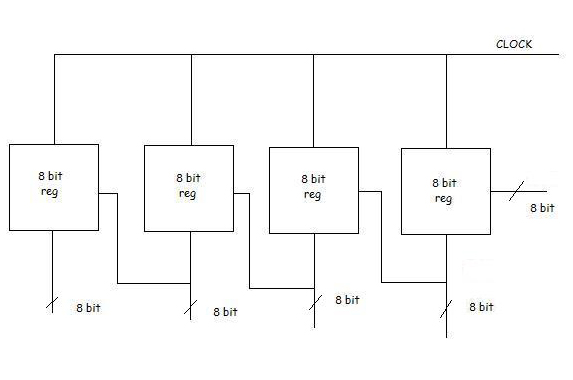
\includegraphics[width = 4in]{./images/shiftregister.jpg}
\caption{Converter using a 8-bit Shift Register}
\end{figure}


% Josep, write in here. 

\newpage
\subsection{Design B: Register with Enable}

\begin{figure}[htp]
\centering
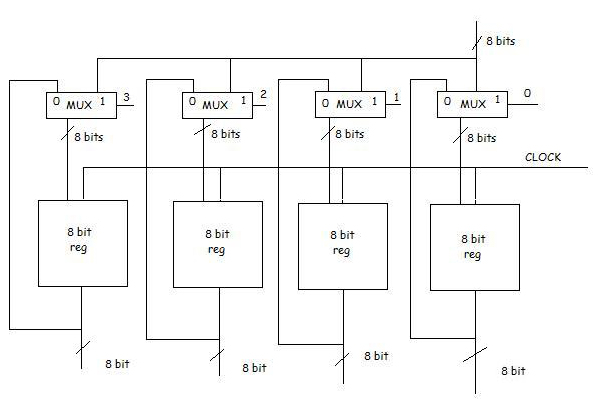
\includegraphics[width = 4in]{./images/shiftregisterenable.jpg}
\caption{Converter using 8-bit Registers with Enable}
\end{figure}

% Josep, write in here. 

\newpage
\subsection{Design C: Register with Clock-Gating}

\begin{figure}[htp]
\centering
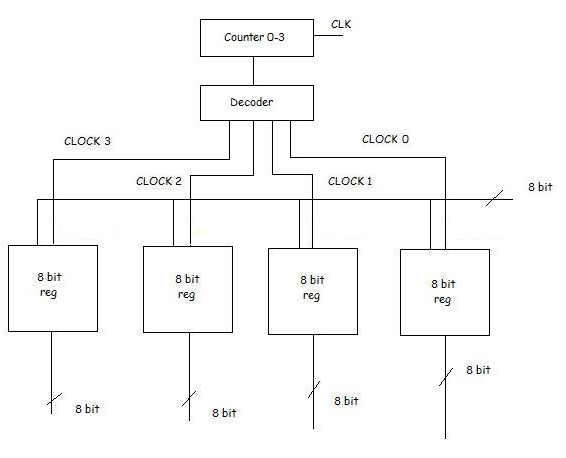
\includegraphics[width = 4in]{./images/shiftregistergated.jpg}
\caption{Converter using 8-bit Registers with Clock Gating}
\end{figure}

% Josep, write in here. 

\newpage
\section{Simulation of the designs with Modelsim}
\label{section:simulation}
All the three designs are simulated with Modelsim, to verify the functionality.
 
The following two screenshots demonstrate the working of implementation for Design A. The first screenshot id taken at 33ns while the second is taken at 43ns. It can be seen that in a new clock cycle, the 8 bit registers ripple their values to the more significant register, and the value of Qk for that clock cycle is fed into the least significant register.

\begin{figure}[htp]
\centering
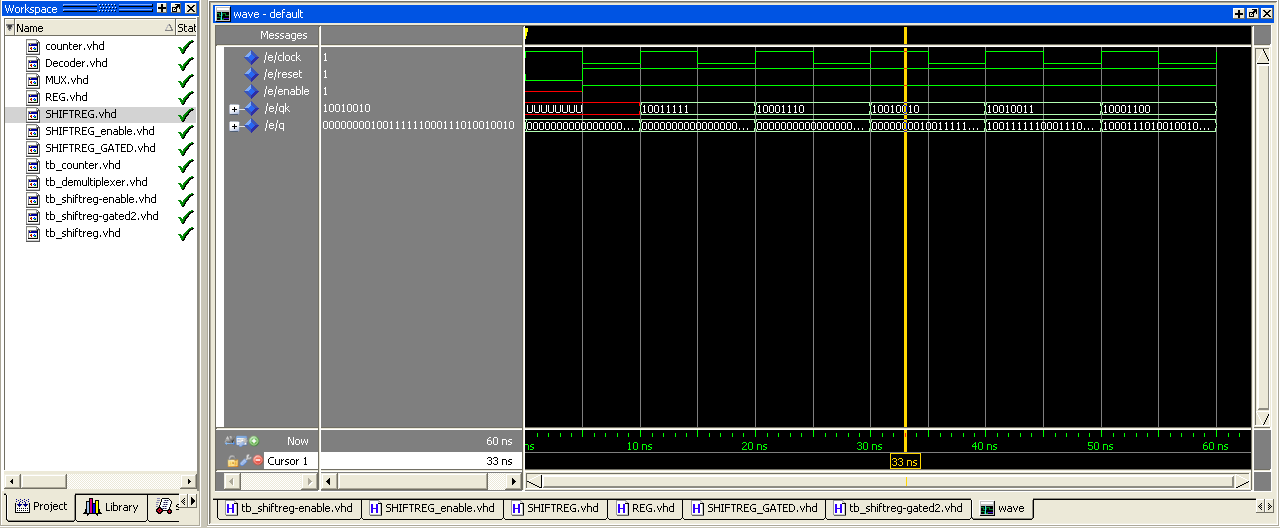
\includegraphics[length = 4in,width = 6.5in]{./images/simsr1.png}
\caption{Simulation screenshot for Design A at 33ns}
\end{figure}

\begin{figure}[htp]
\centering
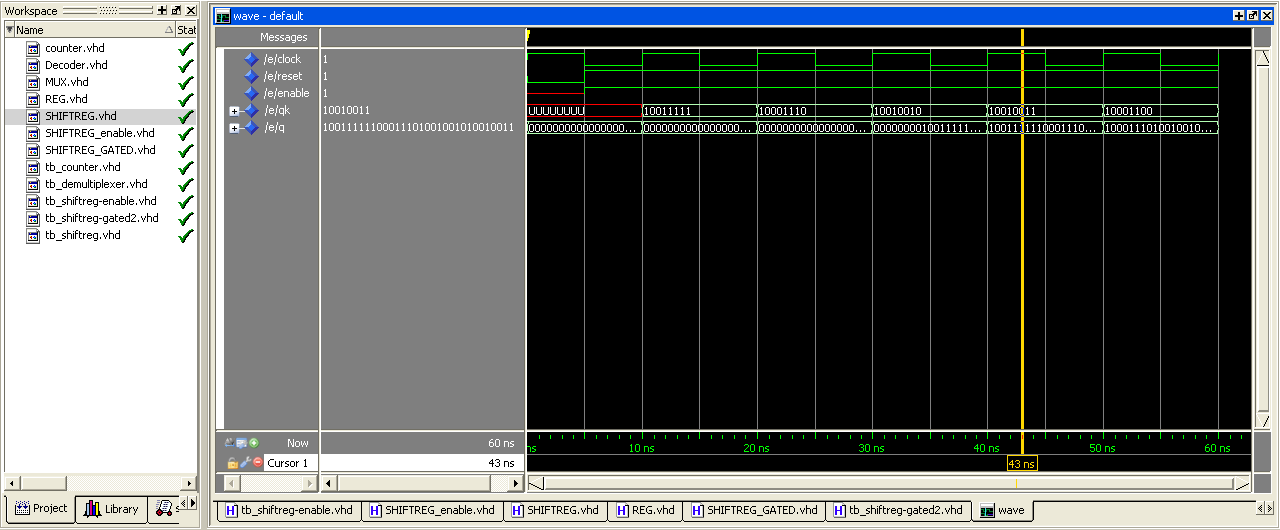
\includegraphics[length = 4in,width = 6.5in]{./images/simsr2.png}
\caption{Simulation screenshot for Design A at 43ns}
\end{figure}

\newpage
The following screenshots are from the simulation of Design B. In the first instance, which is at 14ns on the timeline, we have some value at Qk, but no value at Q. Then, at 24ns, the value of Qk in the previous clock cycle is loaded into the most significant register. Further on, at 33ns, the value of Qk in the previous clock cycle is loaded into the second most significant register. This repeats for four clock cycles.

\begin{figure}[htp]
\centering
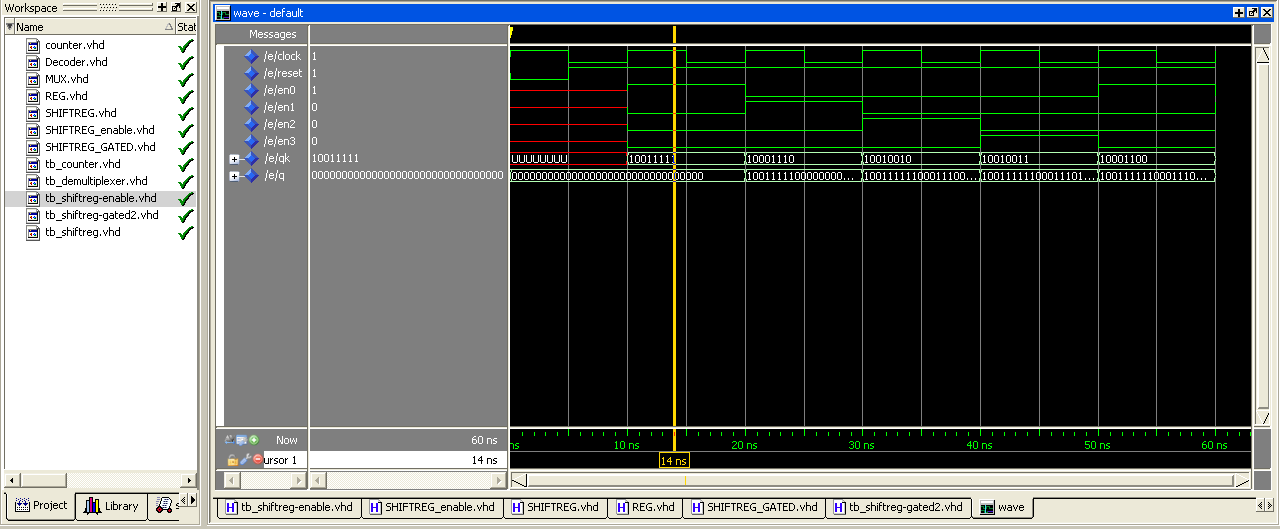
\includegraphics[length = 4in,width = 6.5in]{./images/simsre1.png}
\caption{Simulation screenshot for Design B at 14ns}
\end{figure}

\begin{figure}[htp]
\centering
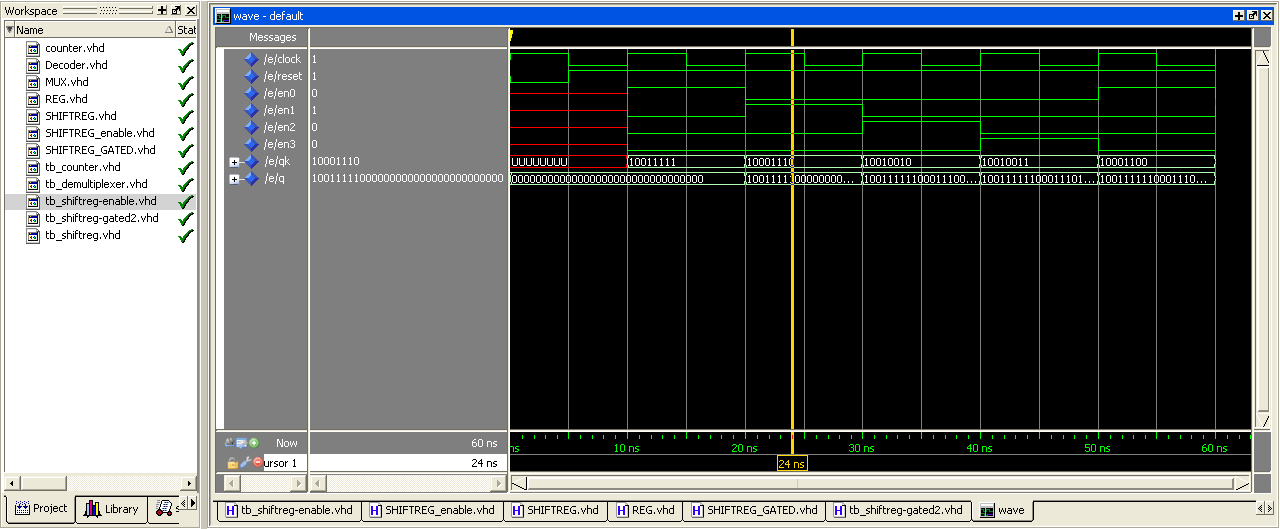
\includegraphics[length = 4in,width = 6.5in]{./images/simsre2.png}
\caption{Simulation screenshot for Design B at 24ns}
\end{figure}

\begin{figure}[htp]
\centering
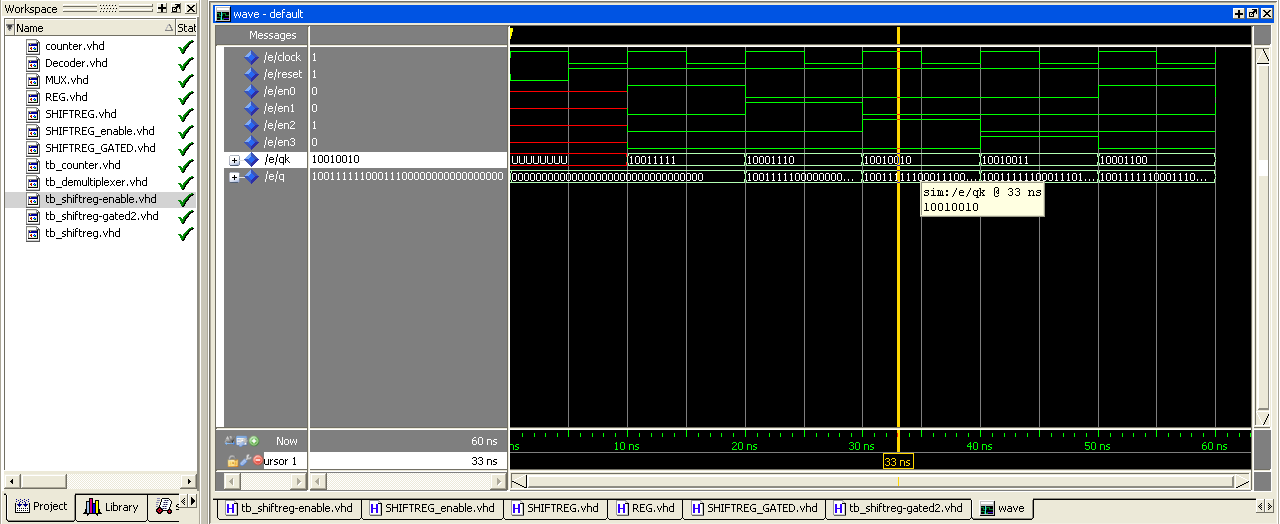
\includegraphics[length = 4in,width = 6.5in]{./images/simsre3.png}
\caption{Simulation screenshot for Design B at 33ns}
\end{figure}

\newpage
Then, for Design C, we have the following screenshots. As we can see, the values of Qk are transferred to the output to different registers. Also, the values of Qk are transferred in the same clock cycle, which was not the case with the Design B.

\begin{figure}[htp]
\centering
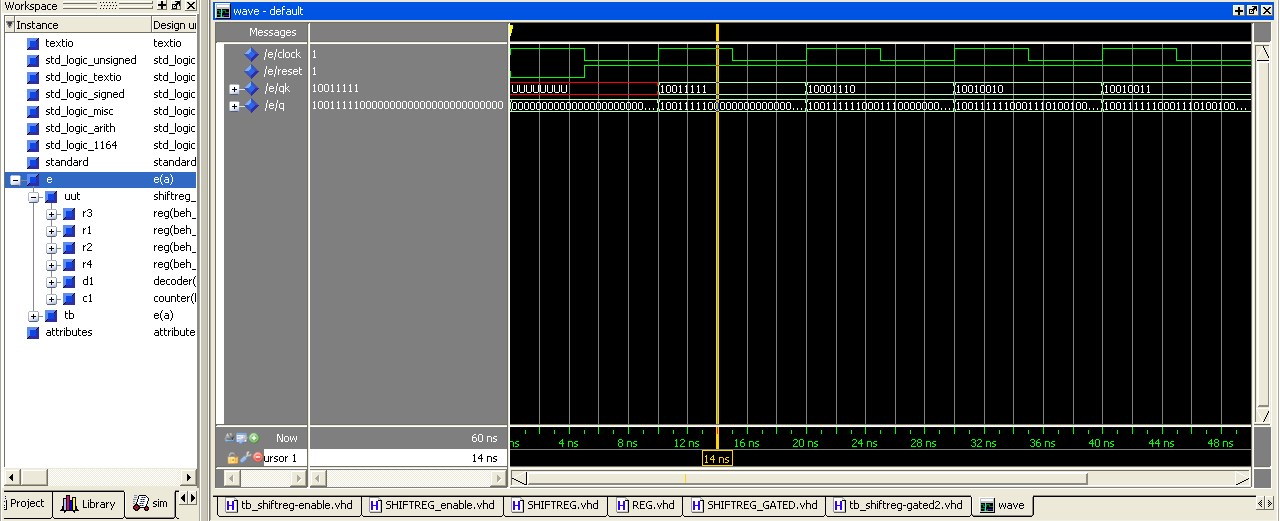
\includegraphics[length = 4in,width = 6.5in]{./images/simsrg1.png}
\caption{Simulation screenshot for Design C at 14ns}
\end{figure}

\begin{figure}[htp]
\centering
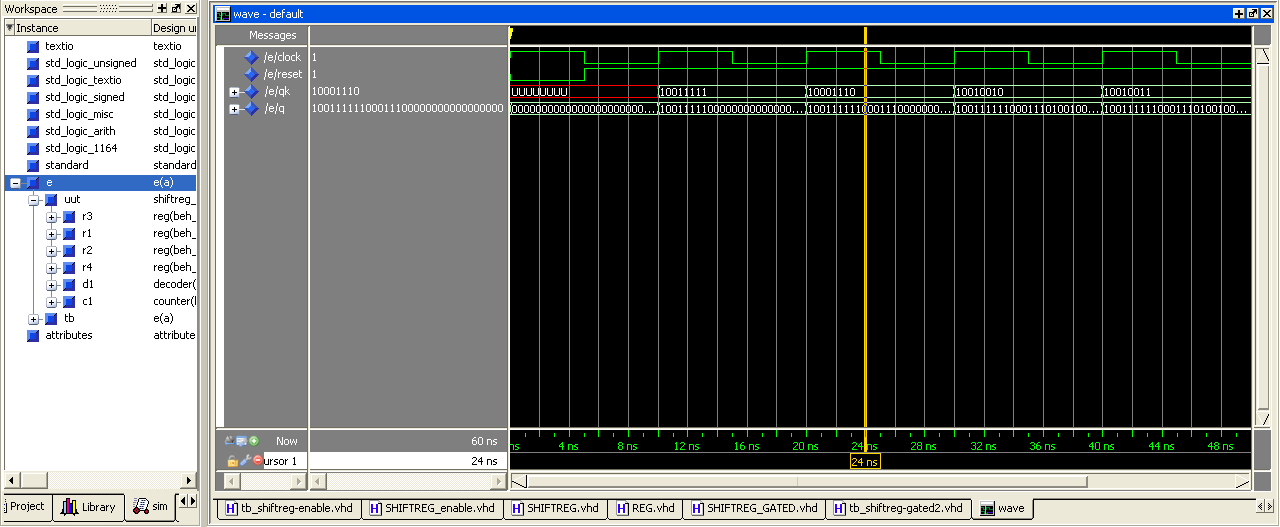
\includegraphics[length = 4in,width = 6.5in]{./images/simsrg2.png}
\caption{Simulation screenshot for Design C at 24ns}
\end{figure}

\newpage
\section{Power Reports and Discussion}
\label{section:power}



\begin{table}[htbp]
\begin{center}
\begin{tabular}{|l|l|l|}
\hline
\textbf{Parameters}	& \textbf{Values}		& \textbf{Comment}\\ \hline
Dynamic Power				&	5.91 mW				& MET\\ \hline
Leakage Power 			&	11.04 uW			& MET\\ \hline
Library Setup Time  & 0.08 ns				& - \\ \hline
Data Arrival Time		& 0.43 ns				& - \\ \hline
SLACK								& -0.01 ns			& VIOLATED \\ \hline
Combinational Area	& 2700 um^2			& - \\ \hline
Non-Combinational Area	& 1343 um^2	& - \\ \hline
SVT cells						& 403						& - \\ \hline
HVT cells						& 0							& - \\ \hline
\end{tabular}
\end{center}
\caption{Clock time-period 0.5 ns, normal power}
\label{tab:syn0.5.1}
\end{table}





\newpage
\section{Implementation and Reports}
\label{section:impl}

\lstinputlisting[frame=trbl, caption={SHIFTREG.vhd}]{../code/SHIFTREG.vhd}
\newpage
\lstinputlisting[frame=trbl,caption={SHIFTREG\_ENABLE.vhd}]{../code/SHIFTREG_ENABLE.vhd}
\newpage
\lstinputlisting[frame=trbl,caption={SHIFTREG\_GATED.vhd}]{../code/SHIFTREG_GATED.vhd}
\newpage
\lstinputlisting[frame=trbl,caption={REG.vhd}]{../code/REG.vhd}
\lstinputlisting[frame=trbl,caption={MUX.vhd}]{../code/MUX.vhd}
\newpage
\lstinputlisting[frame=trbl,caption={COUNTER.vhd}]{../code/counter.vhd}
\lstinputlisting[frame=trbl,caption={DECODER.vhd}]{../code/DECODER.vhd}
\newpage
\lstinputlisting[frame=trbl, caption={Power Report Design A}]{../code/power_report1.txt}
\newpage
\lstinputlisting[frame=trbl, caption={Power Report Design B}]{../code/power_report2.txt}
\newpage
\lstinputlisting[frame=trbl, , caption={Power Report Design C}]{../code/power_report3.txt}
\end{document}